\section{Robot Design}
\label{sec:robot_design}

This is where we explain "overall" design. It's motivation, etc. 
Also where we cover dimensioning, link-lengths, etc. 
We explain here our parameter sweep to find optimal design. 
We also explain here our kinematics-script that we used to derive the required stall-torque for our motor given springs and link-lengths. 

\subsection{The Single Vertical Manipulator Jump Model}

In the absence of air resistance, which is negligible for a robot like this during a jumping maneuver like this, the factor that determines jumping distance is body velocity at takeoff. To keep things simple, in the following will be given an example where the sole goal is to maximize vertical jump height. Further, only a one leg robot with a 2 DOF leg with equal link lengths is considered. 

For a robot such as the one described above, the position of the paw relative to the body can be described by the standard 2 link manipulator equation as seen in equation \ref{eq:2_link_manipulator}, in accordance with the theory in section \ref{sec:robot_kinematics}. For this simple robot, it is assumed that the optimal jump is one where the body center of mass and paw position move in opposite directions, with velocities strictly along the up/down y axis. This example is illustrated in figure \ref{fig:vertical_manipulator}. As is obvious from the figure and from the kinematics, for such a jump $\theta_1 = -\frac{(\theta_2+\pi)}{2}$, and $\dot{\theta}_2=-2\dot{\theta}_1$. If this is combined with the jacobian for the end effector, given in equation \ref{eq:jacobian_vertical_jump_leg}, one can plot the vertical velocity of the paw as a function of the knee angle $\theta_2$, this is shown in figure \ref{fig:vertical_jacobian_velocity}. This is done using the jacobian as in equation \ref{eq:jacobian_speed_mapping}. 

As can be seen in figure \ref{fig:vertical_jacobian_velocity}, the joint velocity of the leg much more readily translates to body velocity when the knee is crouched. Without giving a detailed derivation, the intuition meant to be gained from figure \ref{fig:vertical_jacobian_velocity} is that how quickly the leg joints are accelerated can be just as important as the speed it is accelerated to. This has an important interpretation for the choice of motors, in the sense that, if a given motor is unable to accelerate the leg joints quickly enough, there is little sense in looking for a faster motor, unless it is also stronger. 

\begin{figure}[h]
    \centering
    \includegraphics[width=0.75\textwidth]{Images/vertical_manipulator.png}
    \caption{The manipulator corresponding to a vertical one leg jump.}
    \label{fig:vertical_manipulator}
\end{figure}

\begin{equation}
    \label{eq:2_link_manipulator}
    \begin{aligned}
        x_{\text{end}} &= L_1 \cos(\theta_1) + L_2 \cos(\theta_1 + \theta_2) \\
        y_{\text{end}} &= L_1 \sin(\theta_1) + L_2 \sin(\theta_1 + \theta_2)
    \end{aligned}
\end{equation}

\begin{equation*}
    \label{eq:jacobian_vertical_jump_leg}
    J = \begin{bmatrix} 
    -L_1 \sin(\theta_1) - L_2 \sin(\theta_1 + \theta_2) & -L_2 \sin(\theta_1 + \theta_2) \\
    L_1 \cos(\theta_1) + L_2 \cos(\theta_1 + \theta_2) & L_2 \cos(\theta_1 + \theta_2)
    \end{bmatrix}
\end{equation*}

\begin{figure}[h]
    \centering
    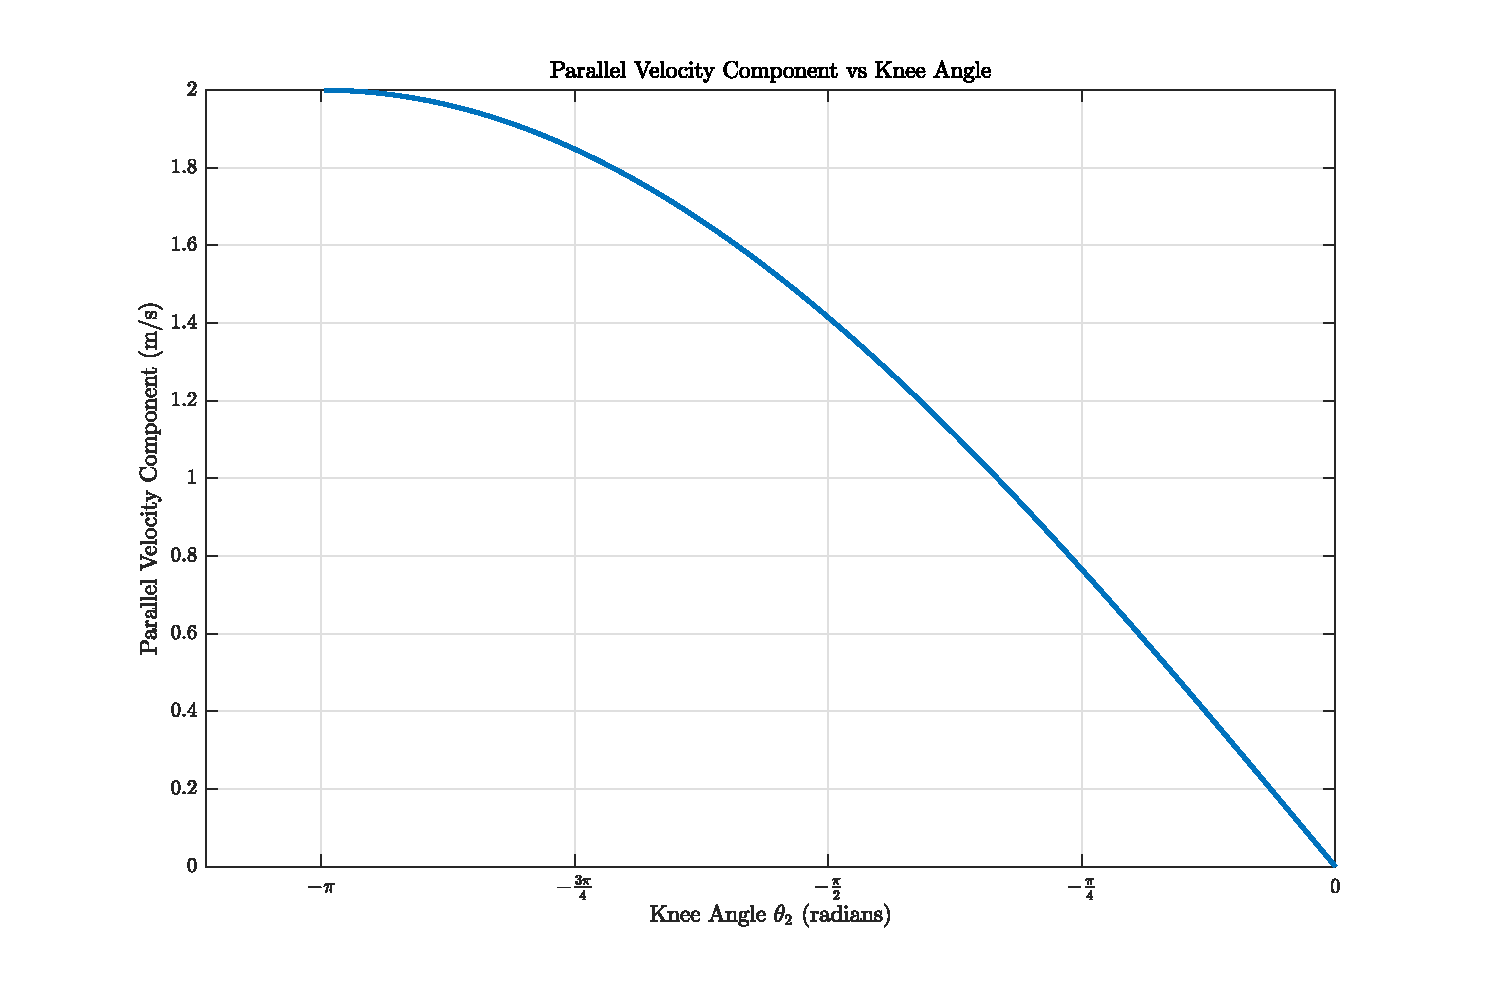
\includegraphics[width=0.75\textwidth]{Images/vertical_jacobian_velocity.eps}
    \caption{Vertical Paw velocity as a function of knee angle.}
    \label{fig:vertical_jacobian_velocity}
\end{figure}

\subsection{Actuation Method Selection: Motors Only}

One of the most central decisions that had to be made for the robot was the choice of actuation method. The two main options considered were to use motors alone, or to use a combination of motors and springs, this section covers our attempts to do the former. 

Initially, experiments were done utilizing motors alone. Due to the need for a light and strong motor, a series of AGF-RC motors were chosen. These motors were chosen due to their high torque to weight ratio. While extensive testing was done, the jumping performance was so far from acceptable that not too much detail will be presented here. The best jumping performance was achieved with the A80BHP-H motor from AGF-RC. This motor has a stall torque of 18.5 kg/cm, a weight of 80 grams, and a maximum velocity of 2000 degrees per second. To test jumping performance, the robots dimensions were gradually increased, body length as well as link lengths. This gradual increase was terminated when the body length reached 30cm and the thigh and shank links reached 20cm each, for a total leg length of 40cm. The search was terminated here because the robot was still not jumping satisfactorily, despite the robots dimensions having reached a point where they were considered excessive. Primarily because the body mass was not being scaled with the general dimensions of the robot, and because the jump height was also not increasing at a commensurate rate with the increase in robot size. Ie., even though the total center of mass displacement was increasing, the center of mass jump height compared to the total length of the legs was not increasing, and the robot was thus not jumping higher. The achieved velocity of the knee joint until takeoff can be seen in figure \ref{fig:joint_speed_A80BHM}. As can be seen, the motor torque drops quickly, and is not able to reach a high enough speed to achieve a good jump. In fact, the peak body center of mass height reached is 70cm, despite a total leg length of 40cm. As can be seen, the motor is too slow to reach a high enough joint velocity for a good jump, it is therefore unlikely that a faster but weaker motor would perform much better. Efforts were made to test motors with both higher torques and higher speeds, but no motors were found with similar specs without being significantly heavier and larger. TODO: Should I show some motors that are objectively worse, as an example? 

\begin{figure}[h]
    \centering
    \includegraphics[width=0.75\textwidth]{Images/joint_speed_A80BHM.eps}
    \caption{Knee speed until takeoff with A80BHP-H motor.}
    \label{fig:joint_speed_A80BHM}
\end{figure}

\subsection{Actuation Method Selection: Motors and Torsional Spring}

The next actuation method considered was to use a combination of motors and torsional springs, as this is the design we ended up choosing, a CAD model of this design can be seen in figure TODO: 

\subsection{}